\chapter{Detalles de Implementación y Experimentos}\label{chapter:implementation}
En este capítulo se aborda la implementación de cada uno de los componentes que conforman el \emph{pipeline}
descrito en la propuesta de solución.

\section{Carga de documentos}
La carga de documentos se realiza haciendo uso de la biblioteca \emph{langchain} [\cite{langchain}],
en particular del submódulo \emph{PyPDFLoader} del módulo \emph{document\_loaders}. Este módulo puede ser sustituido por otro módulo siempre que la respuesta cuente con campos \emph{metadata} y \emph{page\_content}. En caso de sustituir completamente el módulo de carga de documentos se debe garantizar que como resultado del primer paso se tengan dos listas, una con el texto de los documentos y otra con los metadatos correspondientes.
    \subsection{Segmentación del texto}
        Una de las limitaciones tanto de los modelos de \emph{embedding} como de los \emph{LLM} es la cantidad máxima de tokens\footnote{Un \emph{token} se refiere a una unidad individual de significado en un texto.} que puede procesar de una vez. Por ello es necesario, para documentos muy extensos, realizar una segmentación del texto y procesarlos parcial e independiente de las partes.
        En la implementación asociada a esta investigación se incluye tanto la segmentación por oraciones como la segmentación por párrafos, no obstante puede que algunos párrafos excesivamente extensos, saturen la capacidad máxima del modelo. Toda vez que se encuentren cargados y segmentados los documentos, cada segmento de texto se asocia con los metadatos correspondientes

\section{Transformación a vectores}
    \subsection{Modelo para la generación de \emph{embeddings}}
        Para la implementación de este \emph{pipeline} se utilizó un conjunto de modelos de generación de \emph{embeddings} comprendidos entre las 15 primeras posiciones proporcionadas por \emph{MTEB} [\cite{leaderboard}] al momento de la revisión.

        Las dimensiones de los vectores generados por estos modelos de embedding varían entre los 1024, 768 y 384 elementos; la longitud de la secuencia que pueden procesar en todos los casos es de 512. Con la selección de modelos con características diferentes se pretendió determinar si el desempeño de dichos modelos esta directamente ligado a los resultados del modelo arrojados por \emph{MTEB}, de igual manera se persiguió evaluar las diferencias en la calidad del desempeño de un modelo extenso en comparación con uno más limitado.

    Para la implementación del modelo de vectorización se creó una clase \emph{Embeddings} que va a actuar a modo de \emph{wrapper}\footnote{Un \emph{wrapper} es un programa o código que encapsula y facilita el uso de otros componentes del programa}. En la implementación proporcionada se utilizó la biblioteca \emph{langchain} [\cite{langchain}], particularmente el módulo de \emph{embeddings} de HuggingFace para cargar los modelos de \emph{embeddings}. Y se definen los métodos siguientes:
    \begin{enumerate}
        \item \emph{encode\_many}: Método que recibe una lista de documentos y retorna una lista con los vectores resultantes del procesamiento de dicho documento
        \item \emph{encode}: Método que recibe una cadena de texto y retorna el vector resultante del procesamiento  de dicho documento 
        \item \emph{get\_model}: Método que retorna el modelo de \emph{embeddings} que fue cargado. Esto es necesario para que tenga consistencia la búsqueda de similaridad de la base de datos
    \end{enumerate}

    Esta clase forma parte del \emph{pipeline}, no obstante puede ser reemplazada por otra implementación que sea consecuente con el diseño descrito.

    \subsection{Base de Datos Vectorial}
        \subsubsection{Selección del sistema de bases de datos}
            El sistema de bases de datos seleccionado para este proyecto es \emph{ChromaDB} [\cite{chromadb}]. Chroma DB es una base de datos vectorial que se destaca por su eficiencia en el almacenamiento y recuperación de vectores de \emph{embeddings}. Permite la creación de colecciones, el filtrado de texto y la consulta de documentos similares, además de tener una excelente integración con python.
        Las interacciones con la base de datos se hacen a través de una clase que actúa a modo de \emph{wrapper}, esta vez con la siguiente estructura:
        \begin{enumerate}
            \item \emph{create\_collection}: crea una nueva colección en la base de datos.
            \item \emph{get\_collection}: retorna una colección, las operaciones se realizan sobre las colecciones.
            \item \emph{list\_collections}: retorna una lista con todas las colecciones existentes.
            \item \emph{add} añade a la base de datos un nuevo documento, lo vectoriza utilizando el modelo de \emph{embeddings} definido. Si no se define ninguno, utiliza por defecto el modelo \emph{`all-MiniLM-L6-v2'} de \emph{SentenceTransformers}. Recibe como entrada el texto del documento y los metadatos.
            \item \emph{add\_embedding\_to\_database}: añade un nuevo documento que ya haya pasado por el proceso de \emph{embedding}. Recibe como entrada el texto del documento, el vector que lo representa y los metadatos.
            \item \emph{add\_embeddings}: añade un grupo de documentos ya vectorizados a la base de datos. Recibe como entrada el texto del documento, los vectores y los metadatos. 
            \item \emph{query}: realiza una búsqueda de documentos relevantes para una consulta. La entrada será el texto  de la consulta y retorna los documentos relevantes. Con vectores, texto y metadatos, la consulta es vectorizada por el modelo de \emph{embeddings} definido.
            \item \emph{query\_embeddings}: tiene un comportamiento similar a \emph{query} pero recibe en vez del texto a vectorizar, el vector que los representa; retorna los documentos relevantes (texto, vectores, metadatos).
        \end{enumerate}

        Todos los métodos de recuperación de información tienen un parámetro opcional \emph{top\_k} que define la cantidad de documentos a retornar.

        Los métodos de inserción comprenden un mecanismo que revisa si existen ya en la base de datos otros documentos que puedan ser redundantes con el nuevo documento que se desea insertar. La similaridad máxima permitida entre dos vectores es 0.9. No obstante, este valor es modificable para tener un mayor control sobre el criterio de similaridad, en correspondencia con el modelo de \emph{embeddings} que se utilice.

        Este módulo, como los demás del \emph{pipeline}, es reemplazable por otros personalizados siempre que sean consecuentes con la \emph{API}\footnote{Una \emph{API} (Interfaz de Programación de Aplicaciones) es un conjunto de definiciones y protocolos que permite a diferentes aplicaciones comunicarse entre sí y compartir información y funcionalidades.} descrita.

\section{Detección de temas}
    El proceso de detección de los temas (\emph{Topic Modelling}) se realiza a través de un proceso de agrupamiento o \emph{clustering}\footnote{El \emph{clustering} o análisis de agrupamiento es una técnica de aprendizaje no supervisado que agrupa un conjunto de datos en diferentes grupos o cl\'usteres} en el espacio de vectores que comprende los vectores que representan los documentos.

    \subsection{Algoritmo de \emph{Clustering}}
        Para este proceso se utiliza el algoritmo \emph{K-Means Clustering}, en particular la implementación que ofrece \emph{SKLearn} [\cite{sklearn}] que además del algoritmo en sí, ofrece un método de detección automática de la cantidad óptima de cl\'usteres a través del método del codo [\cite{elbow}].
    
    Se implementó un \emph{wrapper} para este proceso, que comprende los siguientes métodos:
    \begin{enumerate}
        \item \emph{generate\_embeddings}: Método para procesar los documentos en caso de que no se proporcionen las versiones vectorizadas de estos. Retorna la lista de vectores correspondiente a los \emph{embeddings} de los documentos.
        \item \emph{detect\_outliers}: Detecta los vectores que pueden ser considerados \emph{outliers}\footnote{En estadística, un \emph{outlier} es un punto de datos que difiere significativamente de otras observaciones} para evitar que estos afecten la correcta posición de los centroides.
        \item \emph{detect\_optimal\_k}: Detecta la cantidad óptima de temas para agrupar los datos acorde al método del codo. La cantidad de grupos, por defecto, se encuentra en el rango entre 2 y 15; no obstante, estos valores pueden ser modificados a través de los parámetros \emph{lim\_sub} y \emph{lim\_sup} de la función.
        \item \emph{topic\_words}: Retorna las palabras más repetidas en cada cl\'uster; retira de la lista de palabras las que están definidas en las \emph{stopwords} de \emph{nltk}\footnote{Módulo \emph{Natural Language Toolkit} https://www.nltk.org}
        \item \emph{get\_topics}: Método principal que recibe los documentos, los procesa y extrae los \emph{outliers}. Al grupo de documentos sin \emph{outliers} les detecta el número óptimo de cl\'usteres. Una vez detectado este número, realiza el proceso de \emph{clustering}. Esta vez con todos los documentos. De los cl\'usteres obtenidos, extrae las palabras representativas y, utilizando un \emph{LLM}, genera una sugerencia de título a partir de estas palabras. Este método retorna el centroide, las palabras más frecuentes y el título sugerido para cada clúster detectado.
    \end{enumerate}

    Este proceso descrito genera una agrupación de los vectores de forma tal que se detectan distintos temas con los cuales asociar la información contenida en los documentos. Los centroides detectados están representados por vectores de la misma dimensionalidad que los vectores generados en en proceso de \emph{embedding}. Si se hiciera una representación en 2D del proceso descrito se obtendría una representación similar a la Figura 2 
    \begin{figure}
        \centering
        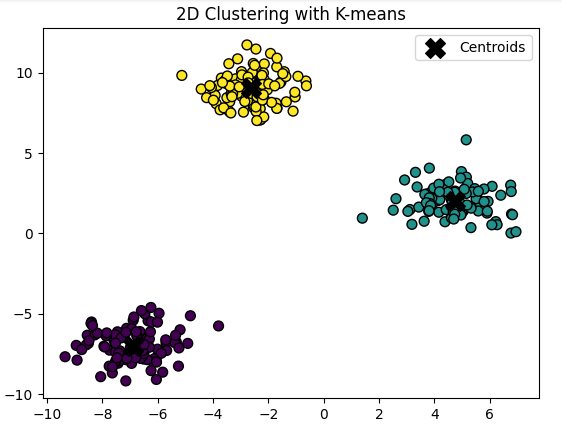
\includegraphics[scale = 0.7]{Figures/clustering.png}
        \caption*{Figura 2: Representación en 2D de un corpus donde se identifican claramente 3 temas}
    \end{figure}
    donde los puntos con color simbolizan los documentos asociados a un tema  y las cruces negras los centroides de cada uno de los temas.

    De esta manera si el centroide representa el punto que define la pertenencia de los documentos a un clúster  que a su vez representa un tema, al obtenerse los documentos más relevantes con relación al vector que representa el centroide se estarán obteniendo los documentos más relevantes para el tema representado por dicho clúster . Esto tendría una correspondencia directa con la calidad de la representación vectorial del modelo de embeddings utilizado.
\section{Generación de los resúmenes}
    Una vez obtenidos los clústeres  se utilizan los centroides para recuperar los documentos más relevantes para cada tema. En este paso es importante tener en cuenta el método de segmentación de texto que se utilizó en el paso de carga de documentos. Este determinaría la cantidad de documentos a recuperar para, consecuentemente, no obtener una cantidad de documentos superior o inferior a la deseada, pues esto podría afectar la calidad de los resúmenes generados.
    
    Estos documentos recuperados, conforman un resumen extractivo preliminar, que a su vez es utilizado como parte del \emph{prompt} de un \emph{LLM} para generar una abstracción del mismo. De esta manera se obtiene una lista de los resúmenes de cada una de las secciones con las que se generará el estado del arte asociado a esos documentos, en correspondencia con la plantilla definida.
    Los documentos recuperados que son utilizados para generar el resumen de cada tema contienen en sus metadatos la información suficiente para identificar a qué archivo del corpus pertenecen. Así se añaden las referencias a estos documentos de origen, utilizando dicha información, que coadyuva a la constucción de las referencias bibliográficas del estado del arte generado.


\section{Plantilla de Estado del Arte}
Se define la plantilla de estado del arte como un documento con formato enumerativo de los temas descubiertos. Para cada elemento se obtiene:
\begin{enumerate}
    \item Título sugerido para el tema
    \item Texto con la información generada y las referencias a las citas bibliográficas
    \item Bloque con la bibliografía (a modo de citas) de los documentos de los que se obtuvo la información
\end{enumerate}

Esta plantilla es una definición del formato del documento que se genera con la información resultante de la ejecución del \emph{pipeline} en un corpus de documentos.

\section{Experimentación y validación}
Para el proceso de validación se utilizaron las m\'etricas (P, R y F1)\footnote{\emph{P (precisión)}: Es una medida que se define como a la fracción de instancias recuperadas que son relevantes. \emph{R (recobrado)}: M\'etrica que inidca cu\'antos de los documentos relevantes fueron identificados correctamente \emph{F1}: El valor F se considera como una media armónica que combina los valores de la precisión y recobrado} reportadas por \emph{BERTScore} [\cite{bertscore}] al evaluar los resultados del \emph{pipeline}.
Para la evaluación se utilizaron los \emph{datasets} \emph{Mult-X-Science} [\cite{multixscience}] enfocado en la generación de textos a modo de estado del arte basado en abstracts de documentos científicos. Y \emph{WikiAsp} [\cite{wikiasp}] que contiene resúmenes enfocados en diferentes puntos de interés acerca de un tema.

La experimentación fue realizada en la paltaforma \emph{Google Colab} utilizando la configuración con GPU de 16GB \emph{Nvidia V100} dicha experimentación tardó aproximadamente 13 y 7 horas en los \emph{datasets} descritos. En las tablas 3.1 y 3.2 se presentan los resultados preeliminares del desempeño en dichos \emph{datasets}, es importante recalcar la ausencia de \emph{datasets} que se ajusten en extensión al problema.

\begin{table}[htb]
    \centering
    \label{tab:example}
    \begin{tabular}{*6c}
      \toprule
      \multicolumn{2}{c}{P}  & \multicolumn{2}{c}{R} & \multicolumn{2}{c}{F1} \\ \cmidrule(r){1-2} \cmidrule(r){3-4} \cmidrule(l){5-6}
      Mean & Median  &  Mean & Median &     Mean & Median   \\
                                                      
      \bottomrule
    \end{tabular}
    \caption{Resultados de la evaluación en \emph{Multi-X-Science}}

  \end{table}

  \begin{table}[htb]
    \centering
    \label{tab:example}
    \begin{tabular}{*6c}
      \toprule
      \multicolumn{2}{c}{P}  & \multicolumn{2}{c}{R} & \multicolumn{2}{c}{F1} \\ \cmidrule(r){1-2} \cmidrule(r){3-4} \cmidrule(l){5-6}
      Mean & Median  &  Mean & Median &     Mean & Median   \\
                                                      
      \bottomrule
    \end{tabular}
    \caption{Resultados de la evaluación en \emph{WikiAsp}}

    
  \end{table}